In this section the experimental validation is presented.
%
Specifically, we show that by explicitly controlling the diversity in DE, results of state-of-the-art algorithms
are improved further.
%
Particularly, the benchmarks of \CEC{} 2016 and \CEC{} 2017 are considered.
%
Each one of them is composed of thirty different problems.
%
The state-of-the-art is composed by the algorithms that attained the first places of each year competition.
%
Additionally, the standard \DE{} was included.
%
Thus, the algorithms considered from the \CEC{} 2016 are UMOEAs-II \cite{elsayed2016testing} and L-SHADE-EpSin \cite{awad2016ensemble} that achieved 
the first and second place respectively.
%
Similarly, the top algorithms from \CEC{} 2017 are EBOwithCMAR \cite{kumar2017improving} and jSO \cite{brest2017single}.
%
It is interesting to remark that EBOwithCMAR is considered as an improvement of the UMOEAs-II.
%
Additionally, jSO and L-SHADE-EpSin belong to the SHADE's family.
%
All these algorithms are tested with both benchmarks as it is suggested by \cite{molina2017analysis}.

Given that all of them are stochastic algorithms, each execution was repeated 51 times with different seeds.
%
In every case, the stopping criterion was set to $25,000,000$ functions evaluations.
%
We performed our evaluation following the guidelines of \CEC{} benchmark competitions and statistical tests proposed in~\cite{Joel:StatisticalTest}.
%
%Also, we took into account statistical tests.
%
The first one, considers a composed score between the mean of difference error and the rank of the algorithms.
%
The second one, follows a statistical scheme, which applies pair-comparisons based in the distribution of the error between the algorithms.
%
Specifically, if the gap between the values of the best solution found and the optimal solution was $10^{-8}$ or smaller, the error is treated as $0$.
%
%The minimal tolerance to consider a determined problem solved is $1e-8$, hence if the difference of the optimal obtained and the true optinal is below this tolerance then the error is zero.
%
The parameterization indicated by the authors was used in every algorithm and it is as follows:
\begin{itemize}
\item \textbf{EBOwithCMAR}: For EBO, the maximum population size of $S_1 = 18D$, minimum population size of $S_1 = 4$, maximum population size of $S_2 = 146.8D$, minimum population size of $S_2 = 10$, historical memory size H=$6$. For CMAR Population size $S_3 = 4 + 3log(D)$, $\sigma=0.3$, CS = $50$, probability of local search $pl = 0.1$ and $cfe_{ls} = 0.4* FE_{max}$.
\item \textbf{UMOEAs-II}: For MODE, maximum population size of $S_1 = 18D$, minimum population size of $S_1 = 4$, size memory H=$6$. For CMA-ES Population size $S_2 = 4 + \lfloor 3log(D) \rfloor$, $\mu=\frac{PS}{2}$, $\sigma=0.3$, CS = $50$. For local search, $cfe_{ls} = 0.2 * FE_{max}$.
\item \textbf{jSO}: Maximum population size = $25log(D)\sqrt{D}$, historical memory size H= $5$, initial mutation memory $M_F = 0.5$, initial probability memory $M_{CR} = 0.8$, minimum population size = $4$, initial p-best = $0.25*N$, final p-best = $2$.
\item \textbf{L-SHADE-EpSin}: Maximum population size = $25log(D)\sqrt{D}$, historical memory size H= $5$, initial mutation memory $M_F = 0.5$, initial probability memory $M_{CR} = 0.5$, initial memory frequency $\mu_F = 0.5$, minimum population size = $4$, initial p-best = $0.25*N$, final p-best = $2$, generations of local search $G_{LS}=250$.
\item \textbf{ DE-EDM}: $D_I = 0.3$, population size = $250$.
\item \textbf{ Standard-DE}: population size = $250$ (operators as \DEEDM{}).
\end{itemize}
%

Our experimental analyses have been performed in base of the difference between the optimal solution and the best obtained solution.
%
In order to statistically compare the results, a similar guideline than the one proposed in~\cite{Joel:StatisticalTest} was used. 
%
First a Shapiro-Wilk test was performed to check whatever or not the values of the results followed a Gaussian distribution. 
%
If, so, the Levene test was used to check for the homogeneity of the variances. 
%
If samples had equal variance, an ANOVA test was done; if not, a Welch test was performed. 
%
For non-Gaussian distributions, the non parametric Kruskal-Wallis test was used to test whether samples are drawn from the same distribution. 
%
An algorithm $X$ is said to win algorithm $Y$ when the differences between them are statistically significant, and the mean and median obtained by $X$ are higher 
than the mean and median achieved by $Y$.

In tables \ref{tab:Summary_CEC2016} and \ref{tab:Summary_CEC2017} a summary of the results obtained for \CEC{} 2016 and \CEC{} 2017 are shown, respectively.
%
The column tagged with ``Always Solved'' shows the number of functions where a zero error was obtained in the 51 runs.
%
Additionally, column tagged with ``At least one time solved'' shows the number of functions that were solved to optimality at least in one run.
%
Practically all functions (28 of them) of the \CEC{} 2017 benchmark were solved with our proposal at least one time.
%
Additionally, 21 functions of the \CEC{} 2016 were also solved.
%
This constrast with the results obtained by state-of-the-art algorithms.
%
They were able to reach optimal values in significantly less functions.
%
In order to confirm the superioriy of \DEEDM{}, pair-wise statisticall test were used.
%
The column tagged with the symbol $\uparrow$ shows the number of times that the superiority of each method could be confirmed, whereas
the column tagged with the symbol $\downarrow$ count the number of cases where the method was inferior.
%
Finally, the number comparisons whose differences were not significant are shown in the column tagged with the symbol $\longleftrightarrow$.
%
%TODO: Poner frases del tipo que fue el que mas veces ganó y el que menos veces perdió
The statistical tests indicate that the \DEEDM{} attained the best results in both years.
%
The number of wins in \CEC{} 2016 and \CEC{} 2017 were $77$ and $88$ respectively.
%
Also the number of losts were of $25$ and $6$ respectively.
%
Additionally, the last place attained in both years was by the L-SHADE-Epsilon with $20$ wins in 2016 and $7$ wins in 2017.
%
%
The last column tagget with ``Score'' shows the analyses proposed in the \CEC{}'s competitions.
%
Particularly, the evaluation method combines two scores defined in the equation (\ref{eqn:total_scores}).
%
%TODO: pasar el score a la última columna y decir que además del análisis se realizó el análisis propuesto en la competición, que se base
%en calcular un score...
%
Thus the final score is composed by the sum $Score = Score_1 + Score_2$.
%
\begin{equation}\label{eqn:total_scores}
\begin{split}
Score_1 &= \left (1 - \frac{SE - SE_{min}}{SE} \right) \times 50, \\
Score_2 &= \left  (1 - \frac{SR - SR_{min}}{SR} \right ) \times 50, \\
\end{split}
\end{equation}
Here, $SE_{min}$ is the minimal sum of errors from all the algorithms, and $SE$ is the sum of error values $SE = \sum_{i=1}^{30} error\_f_i$.
%
Also, $SR_{min}$ is the minimal sum of ranks from all the algorithms, namely the sum of each rank in each function for the considered algorithms $SE = \sum_{i=1}^{30} error\_f_i$.
%
%TODO: remarcar que la nueva propuesta consigue score 100 en ambos casos, confirmando la superioridad que se vio con el resto de análisis realizados, decir
%que significa tener score 100
% 
Principally, our proposal attained the best scores ($100.00$) in both years, showing its superiority.
%
Additionally, the Standard-DE attained good enough results, in fact it got the third and second places in \CEC{} 2016 and \CEC{} 2017 respectively.
%
This shows that the performance of the state-of-the-art algorithms is different considering long-term executions.
%
Specifically, although that in \CEC{} 2017 the L-SHADE-Epsilon algorithm got the lowest number of wins in the statistical test it showed a competitive score.
%
This might occurs since that the statistical scores considers both mean and median errors.
%
Morever, the score considers a rank and mean based in the error.
%

%TODO: Poner Dado que nuestra novedad está en el control de la diversidad, para comprender mejor el comportamiento de la propuesta...

Giving that our proposal is based in the explicitly control of the diversity and with the aim of a better understanding of its behavior in the figure \ref{fig:diversity} is showed the diversity through the elapsed function evaluatons.
%
Particularly, the \DEEDM{} was executed with the functions $f_1$ and $f_{30}$.
%
Specifically, based in their properties the first function is easily solved (unimodal) and the second is one of the most difficult (hybrid).
%
In the left side is showed the diversity of the Elite population.
%
Although there are not constraints in the Elite population to lost the diversity, it seems that in both functions $f_1$ and $f_{30}$ the diversity is implicitly maintained.
%
Similarly, in the right side is showed the diversity of the trial vectors.
%
It shows that the diversity is explicitly maintained as is desired ( i.e. until the $95\%$ of the total function evaluations).

\begin{figure}[t]
\centering
\begin{tabular}{cc}
   \includegraphics[scale=0.23, angle=-90]{img/Diversity_Elite.eps} 
   \includegraphics[scale=0.23, angle=-90]{img/Diversity_Trial.eps} 
\end{tabular}
\caption{ Average \DCN{} of the 51 executions with the problems $f_1$ and $f_{30}$ (\CEC{} 2016 and \CEC{} 2017). The initial distance factor considered corresponds to $D_I=0.3$.}
\label{fig:diversity}
\end{figure}


% Please add the following required packages to your document preamble:
% \usepackage{multirow}
\begin{table}[t]
\centering
\caption{Summary results - \CEC{} 2016}
\label{tab:Summary_CEC2016}
\begin{tabular}{|c|c|c|c|c|c|c|}
\hline
\multirow{2}{*}{\textbf{Algorithm}} & \multirow{2}{*}{\textbf{\begin{tabular}[c]{@{}c@{}}Always \\ solved\end{tabular}}} & \multirow{2}{*}{\textbf{\begin{tabular}[c]{@{}c@{}}At least one\\ time solved\end{tabular}}} & \multicolumn{3}{c|}{\textbf{Statistical Tests}} & \multirow{2}{*}{\textbf{Score}} \\ \cline{4-6}
 &  &  & $\uparrow$ & $\downarrow$ & $\longleftrightarrow $ &  \\ \hline
\textbf{EBOwithCMAR} & 8 & 14 & 35 & 56 & 59 & 50.28 \\ \hline
\textbf{jSO} & 9 & 17 & 47 & 51 & 52 & 55.43 \\ \hline
\textbf{UMOEAs-II} & 9 & 14 & 51 & 31 & 68 & 62.45 \\ \hline
\textbf{L-SHADE-Epsilon} & 7 & 13 & 20 & 71 & 59 & 50.12 \\ \hline
\textbf{DE-EDM} & 13 & 21 & 77 & 25 & 48 & 100.00 \\ \hline
\textbf{Standard-DE} & 11 & 19 & 50 & 46 & 54 & 56.29 \\ \hline
\end{tabular}
\end{table}


% Please add the following required packages to your document preamble:
% \usepackage{multirow}
\begin{table}[t]
\centering
\caption{Summary results - \CEC{} 2017}
\label{tab:Summary_CEC2017}
\begin{tabular}{|c|c|c|c|c|c|c|}
\hline
\multirow{2}{*}{\textbf{Algorithm}} & \multirow{2}{*}{\textbf{\begin{tabular}[c]{@{}c@{}}Always \\ solved\end{tabular}}} & \multirow{2}{*}{\textbf{\begin{tabular}[c]{@{}c@{}}At least one\\ time solved\end{tabular}}} & \multicolumn{3}{c|}{\textbf{Statistical Tests}} & \multirow{2}{*}{\textbf{Score}} \\ \cline{4-6}
 &  &  & $\uparrow$ & $\downarrow$ & $\longleftrightarrow $ &  \\ \hline
\textbf{EBOwithCMAR} & 9 & 18 & 34 & 46 & 70 & 37.14 \\ \hline
\textbf{jSO} & 8 & 15 & 29 & 55 & 66 & 29.30 \\ \hline
\textbf{UMOEAs-II} & 11 & 15 & 43 & 40 & 67 & 26.89 \\ \hline
\textbf{L-SHADE-Epsilon} & 8 & 19 & 7 & 81 & 62 & 32.78 \\ \hline
\textbf{DE-EDM} & 21 & 28 & 88 & 6 & 56 & 100.00 \\ \hline
\textbf{Standard-DE} & 12 & 21 & 56 & 29 & 65 & 42.91 \\ \hline
\end{tabular}
\end{table}



%TODO: Con el fin de que otros autores se puedan comparar con los resultados, reportamos el error alcanzado
In order, to provide comparable results of our proposal, in the tables \ref{tab:Results_CEC2016} and \ref{tab:Results_CEC2017} are reported the best, worst, median, mean, standard deviation and success ratio.
%
Particularly, these tables show that the uni-modal were solved by our proposal.
%
Also, several simple multi-modal functions were adequatelly approximated.
%
Principally, our proposal solved several complex functions (e.g. Composition Functions) that were not solved by the state-of-the-art.
%
\begin{table}[t]
\begin{scriptsize}
\centering
\caption{Results for DE based diversity \CEC{} 2016 problems}
\label{tab:Results_CEC2016}
%\resizebox{\textwidth}{!}{%
\begin{tabular}{|c|c|c|c|c|c|c|}
\hline
 & \textbf{Best} & \textbf{Worst} & \textbf{Median} & \textbf{Mean} & \textbf{Std} & \textbf{Succ. Ratio} \\ \hline
$f_1$ & 0.00E+00 & 0.00E+00 & 0.00E+00 & 0.00E+00 & 0.00E+00 & 1.00E+00 \\ \hline
$f_2$ & 0.00E+00 & 0.00E+00 & 0.00E+00 & 0.00E+00 & 0.00E+00 & 1.00E+00 \\ \hline
$f_3$ & 0.00E+00 & 0.00E+00 & 0.00E+00 & 0.00E+00 & 0.00E+00 & 1.00E+00 \\ \hline
$f_4$ & 0.00E+00 & 0.00E+00 & 0.00E+00 & 0.00E+00 & 0.00E+00 & 1.00E+00 \\ \hline
$f_5$ & 0.00E+00 & 0.00E+00 & 0.00E+00 & 0.00E+00 & 0.00E+00 & 1.00E+00 \\ \hline
$f_6$ & 0.00E+00 & 3.60E-02 & 4.00E-03 & 7.39E-03 & 1.15E-02 & 3.92E-01 \\ \hline
$f_7$ & 2.00E-02 & 1.02E-01 & 5.90E-02 & 5.77E-02 & 4.93E-02 & 0.00E+00 \\ \hline
$f_8$ & 0.00E+00 & 0.00E+00 & 0.00E+00 & 0.00E+00 & 0.00E+00 & 1.00E+00 \\ \hline
$f_9$ & 0.00E+00 & 0.00E+00 & 0.00E+00 & 0.00E+00 & 0.00E+00 & 1.00E+00 \\ \hline
$f_{10}$ & 0.00E+00 & 0.00E+00 & 0.00E+00 & 0.00E+00 & 0.00E+00 & 1.00E+00 \\ \hline
$f_{11}$ & 0.00E+00 & 6.00E-02 & 0.00E+00 & 5.88E-03 & 1.90E-02 & 9.02E-01 \\ \hline
$f_{12}$ & 0.00E+00 & 0.00E+00 & 0.00E+00 & 0.00E+00 & 0.00E+00 & 1.00E+00 \\ \hline
$f_{13}$ & 1.00E-02 & 8.00E-02 & 5.00E-02 & 4.67E-02 & 2.60E-02 & 0.00E+00 \\ \hline
$f_{14}$ & 1.00E-02 & 5.00E-02 & 3.00E-02 & 2.82E-02 & 2.13E-02 & 0.00E+00 \\ \hline
$f_{15}$ & 0.00E+00 & 4.70E-01 & 2.20E-01 & 1.99E-01 & 1.55E-01 & 1.96E-02 \\ \hline
$f_{16}$ & 4.00E-02 & 1.50E-01 & 8.00E-02 & 8.47E-02 & 4.96E-02 & 0.00E+00 \\ \hline
$f_{17}$ & 0.00E+00 & 0.00E+00 & 0.00E+00 & 0.00E+00 & 0.00E+00 & 1.00E+00 \\ \hline
$f_{18}$ & 0.00E+00 & 2.00E-02 & 1.00E-02 & 7.65E-03 & 6.32E-03 & 3.14E-01 \\ \hline
$f_{19}$ & 0.00E+00 & 0.00E+00 & 0.00E+00 & 0.00E+00 & 0.00E+00 & 1.00E+00 \\ \hline
$f_{20}$ & 0.00E+00 & 0.00E+00 & 0.00E+00 & 0.00E+00 & 0.00E+00 & 1.00E+00 \\ \hline
$f_{21}$ & 0.00E+00 & 0.00E+00 & 0.00E+00 & 0.00E+00 & 0.00E+00 & 1.00E+00 \\ \hline
$f_{22}$ & 0.00E+00 & 3.00E-02 & 0.00E+00 & 3.73E-03 & 2.76E-02 & 7.65E-01 \\ \hline
$f_{23}$ & 0.00E+00 & 1.00E+02 & 0.00E+00 & 2.55E+01 & 5.10E+01 & 7.45E-01 \\ \hline
$f_{24}$ & 0.00E+00 & 6.90E-01 & 0.00E+00 & 2.61E-02 & 1.33E-01 & 9.61E-01 \\ \hline
$f_{25}$ & 1.00E+02 & 1.00E+02 & 1.00E+02 & 1.00E+02 & 0.00E+00 & 0.00E+00 \\ \hline
$f_{26}$ & 8.00E-02 & 1.00E+02 & 5.29E+01 & 5.20E+01 & 3.19E+01 & 0.00E+00 \\ \hline
$f_{27}$ & 2.50E-01 & 9.10E-01 & 5.40E-01 & 5.60E-01 & 2.92E-01 & 0.00E+00 \\ \hline
$f_{28}$ & 0.00E+00 & 3.57E+02 & 3.43E+02 & 2.76E+02 & 1.60E+02 & 1.96E-01 \\ \hline
$f_{29}$ & 1.00E+02 & 1.00E+02 & 1.00E+02 & 1.00E+02 & 0.00E+00 & 0.00E+00 \\ \hline
$f_{30}$ & 1.84E+02 & 1.84E+02 & 1.84E+02 & 1.84E+02 & 3.25E-02 & 0.00E+00 \\ \hline
\end{tabular}%
%}
\end{scriptsize}
\end{table}

\begin{table}[t]
\begin{scriptsize}
\centering
\caption{Results for DE based diversity \CEC{} 2017 problems}
\label{tab:Results_CEC2017}
%\resizebox{\textwidth}{!}{%
\begin{tabular}{|c|c|c|c|c|c|c|}
\hline
 & \textbf{Best} & \textbf{Worst} & \textbf{Median} & \textbf{Mean} & \textbf{Std} & \textbf{Succ. Ratio} \\ \hline
$f_1$ & 0.00E+00 & 0.00E+00 & 0.00E+00 & 0.00E+00 & 0.00E+00 & 1.00E+00 \\ \hline
$f_2$ & 0.00E+00 & 0.00E+00 & 0.00E+00 & 0.00E+00 & 0.00E+00 & 1.00E+00 \\ \hline
$f_3$ & 0.00E+00 & 0.00E+00 & 0.00E+00 & 0.00E+00 & 0.00E+00 & 1.00E+00 \\ \hline
$f_4$ & 0.00E+00 & 0.00E+00 & 0.00E+00 & 0.00E+00 & 0.00E+00 & 1.00E+00 \\ \hline
$f_5$ & 0.00E+00 & 0.00E+00 & 0.00E+00 & 0.00E+00 & 0.00E+00 & 1.00E+00 \\ \hline
$f_6$ & 0.00E+00 & 0.00E+00 & 0.00E+00 & 0.00E+00 & 0.00E+00 & 1.00E+00 \\ \hline
$f_7$ & 0.00E+00 & 0.00E+00 & 0.00E+00 & 0.00E+00 & 0.00E+00 & 1.00E+00 \\ \hline
$f_8$ & 0.00E+00 & 0.00E+00 & 0.00E+00 & 0.00E+00 & 0.00E+00 & 1.00E+00 \\ \hline
$f_9$ & 0.00E+00 & 0.00E+00 & 0.00E+00 & 0.00E+00 & 0.00E+00 & 1.00E+00 \\ \hline
$f_{10}$ & 0.00E+00 & 1.20E-01 & 0.00E+00 & 1.65E-02 & 3.39E-02 & 7.45E-01 \\ \hline
$f_{11}$ & 0.00E+00 & 0.00E+00 & 0.00E+00 & 0.00E+00 & 0.00E+00 & 1.00E+00 \\ \hline
$f_{12}$ & 0.00E+00 & 2.20E-01 & 0.00E+00 & 6.37E-02 & 1.76E-01 & 6.67E-01 \\ \hline
$f_{13}$ & 0.00E+00 & 0.00E+00 & 0.00E+00 & 0.00E+00 & 0.00E+00 & 1.00E+00 \\ \hline
$f_{14}$ & 0.00E+00 & 0.00E+00 & 0.00E+00 & 0.00E+00 & 0.00E+00 & 1.00E+00 \\ \hline
$f_{15}$ & 0.00E+00 & 0.00E+00 & 0.00E+00 & 0.00E+00 & 0.00E+00 & 1.00E+00 \\ \hline
$f_{16}$ & 0.00E+00 & 2.10E-01 & 0.00E+00 & 2.47E-02 & 7.27E-02 & 8.82E-01 \\ \hline
$f_{17}$ & 0.00E+00 & 0.00E+00 & 0.00E+00 & 0.00E+00 & 0.00E+00 & 1.00E+00 \\ \hline
$f_{18}$ & 0.00E+00 & 1.00E-02 & 0.00E+00 & 1.96E-03 & 4.47E-03 & 8.04E-01 \\ \hline
$f_{19}$ & 0.00E+00 & 0.00E+00 & 0.00E+00 & 0.00E+00 & 0.00E+00 & 1.00E+00 \\ \hline
$f_{20}$ & 0.00E+00 & 0.00E+00 & 0.00E+00 & 0.00E+00 & 0.00E+00 & 1.00E+00 \\ \hline
$f_{21}$ & 0.00E+00 & 0.00E+00 & 0.00E+00 & 0.00E+00 & 0.00E+00 & 1.00E+00 \\ \hline
$f_{22}$ & 0.00E+00 & 0.00E+00 & 0.00E+00 & 0.00E+00 & 0.00E+00 & 1.00E+00 \\ \hline
$f_{23}$ & 0.00E+00 & 3.00E+02 & 0.00E+00 & 3.49E+01 & 1.03E+02 & 8.82E-01 \\ \hline
$f_{24}$ & 0.00E+00 & 0.00E+00 & 0.00E+00 & 0.00E+00 & 0.00E+00 & 1.00E+00 \\ \hline
$f_{25}$ & 0.00E+00 & 1.00E+02 & 0.00E+00 & 3.92E+00 & 2.00E+01 & 9.61E-01 \\ \hline
$f_{26}$ & 0.00E+00 & 0.00E+00 & 0.00E+00 & 0.00E+00 & 0.00E+00 & 1.00E+00 \\ \hline
$f_{27}$ & 0.00E+00 & 3.87E+02 & 3.87E+02 & 2.05E+02 & 2.68E+02 & 1.96E-02 \\ \hline
$f_{28}$ & 0.00E+00 & 0.00E+00 & 0.00E+00 & 0.00E+00 & 0.00E+00 & 1.00E+00 \\ \hline
$f_{29}$ & 1.45E+02 & 2.26E+02 & 2.18E+02 & 1.99E+02 & 4.21E+01 & 0.00E+00 \\ \hline
$f_{30}$ & 3.95E+02 & 3.95E+02 & 3.95E+02 & 3.95E+02 & 2.10E-01 & 0.00E+00 \\ \hline
\end{tabular}%
%}
\end{scriptsize}
\end{table}

\subsection{Empirical analyses of the initial distance factor}

In our proposal the diversity is explicitly promoted through several stages, which are controlled with the initial distance factor $D_I$.
%
Therefore, the effect of this parameter is analysed in detail.
%
Particularly, the general configuration of the experimental validation is taken into account.
%
Thus, several initial distance factors were considered ($D_I = \{0.0, 0.1, 0.2, 0.3, 0.4, 0.5, 0.6, 0.7, 0.8, 0.9, 1.0, 1.1 \}$).
%
\begin{figure}[t]
\centering
  \includegraphics[scale=0.3, angle=-90]{img/Tuning_CEC.eps}
\caption{Average success rate with different initial distance factors in the benchmark of \CEC{} 2016 and \CEC{} 2017, is considered a population size of $250$ and $25,000,000$ function evaluations.}
\label{fig:one}
\end{figure}

In the figure \ref{fig:one} is showed the average success ratio vs. the initial distance factor $D_I$.
%
The most relevant points are described as follows:
\begin{itemize}
\item If the diversity is not promoted ($D_I = 0.0 $) the performance of the algorithms is seriously implicated.
\item In this scenario the ideal configuration is $D_I=0.3$, although that the range $[0.1, 0.4]$ also provides quality solutions.
\item If the diversity of the solutions increases (after a range) the quality of solutions is implicated.
\end{itemize}
Finally, its important stand out that the solutions are less affected by the population size, however there is still present a relation between the $D_I$ and the population size.
%

